\documentclass{article}
\usepackage{tikz}
\usepackage{graphicx}
\usepackage{hyperref}
\usepackage{listings}
\usepackage{float}
\usepackage{pdfpages}


\lstset{frame=tb,
extendedchars = true,
texcl=true,
  language=bash,
  aboveskip=3mm,
  belowskip=3mm,
  showstringspaces=false,
  columns=flexible,
  basicstyle={\small\ttfamily},
  numbers=none,
  numberstyle=\tiny\color{gray},
  keywordstyle=\color{blue},
  commentstyle=\color{dkgreen},
  stringstyle=\color{mauve},
  breaklines=true,
  breakatwhitespace=true,
  tabsize=3
}

\graphicspath{ {./img/} }

\author{Kent Odde, Stian Onarheim, Tarald Vestbøstad}
\title{Title}

\begin{document}

\pagestyle{empty}

 \begin{tikzpicture}[remember picture,overlay]
    \node[anchor=north west,yshift=-15pt,xshift=20pt]%
        at (current page.north west)
        {
\includegraphics[height=8em]{img/USN_logotype.png}};

\end{tikzpicture}


%\vspace{2.5cm}

{\LARGE test}\hspace{2cm}

\begin{tikzpicture}[overlay]
    \node[anchor=north, inner sep=0] at (4,-2)
        {
\includegraphics[width=\textwidth]{img/frontpage-block.png}};
\end{tikzpicture}

\begin{tikzpicture}[overlay]
    \node[anchor=north, inner sep=0] at (-3,-0) {\large Hello};
        
\end{tikzpicture}

\maketitle

\newpage
\tableofcontents

\newpage
\section{Maybe useful text}

Thursday 20. August 2020, the group gathered and had a meeting with Steven Bos. We discussed our project idea and the potential use of the Microsoft HoloLens 2. It was in the group's best interest to put our resources into the microcontroller rather than the goggles, dismissing any development with the HoloLens.

\vspace{5mm}
On September 10. the group met to plan the project. After deciding on the initial design, we drew a sketch and wrote a short description. This was sent to our professor, along with a list of required parts as well as the associated budget. The initial design can be seen in section XX.

\vspace{5mm}

On the 16th of September, we ordered three Arduino Nano 33 BLE Sense w/headers from Arduino.cc. This came to 1080NOK. In addition to this the professor provided us with a car for the project. It is called \href{https://hobbyking.com/en_us/turnigy-trooper-sct-4x4-1-10-brushless-short-course-truck-arr.html?___store=en_us}{Turnigy Trooper}, and was originally a radio controlled car. However everything but the battery and servo motors for thrust and steering, have been stripped away. 

The servo motors are controlled by a pulse-width modulated signal. This means in essence that we send discrete signals, where the signal will rise at a fixed frequency. The length of time the signal is high before going low will determine the behaviour of the servo motors. Luckily for us there is a standard regarding the behaviour generated by a specific pulse width. 

We will need to write a library which will abstract this away in the code. Where the interface for steering will take an angle, and the motor interface will hopefully be able to take a velocity in m/s, where negative numbers will mean going backwards.

\vspace{5mm}
%Litt vanskelig med fortid og nåtid i formuleringa her = p
After Steven showed us a proof of concept that it will be quite doable to base our library for the Arduino Nano on the existing toolchain for NRF52840, we started developing on the 17th of September. However there quickly emerged a problem, as Gnat arm-elf initally only supports ZFP-runtime libraries for this card. This meant that it would only support barebone functionality, and we would never be able to make use of the Ada realtime library, or even multithreading the software. Luckily, there exists support for full ravenscar run-time libraries for the card. We followed the official guide \url{https://github.com/AdaCore/bb-runtimes} \cite{BBRUNTIMES} to generate and build them ourselves.

%Before we could start using Ada's real-time library under runtime, we had to generate the library for our microcontroller nRF52840. We followed the official guide [kilde]\url{https://github.com/AdaCore/bb-runtimes} to generate and build the library. 

\vspace{5mm}
On the 18th of September we improved our library build, by letting the project\_wizard script in Ada drivers library generate the gpr-files for our board automatically. All we had to do was to provide some basic information about the microcontroller, and the script did the rest. We also started adapting the pin mappings from the nrf52832 to the nrf52840. 

Provided that our efforts lead to a useful library, we will create a pull request into the Ada drivers library, so that others may benefit from our work. 


\vspace{5mm}

October 5. 

We received the Segger J-Link debugger from our professor. In order to get this to work, we installed the firmware from segger.com. However we also had to install a pack for pyocd in order to find the debugger:

pyocd pack --install  stm32l476VG

As all development within the group is done on Linux, we also had to add udev rules, so that we were able to access the usb ports without being root. These rule-sets were found on pyocds git repository.

We also had to give the respective user access to the serial port by running the command: 
usermod -a -G dialout MY\_USER\_NAME


Legge til utilization test og grafikk.

\section{Ravenscar}

The full ravenscar run-time library offers what is called the Ravenscar profile. This is a subset of the Ada language, where the features and available libraries are limited. The reason for this is to ensure robust software on realtime and safety critical systems. 

The specifications of the ravenscar profile are the following:
%Lim inn liste kanskje?
https://www.ada-switzerland.ch/rm/RM-D-13.html

There are a couple of limitations here that will affect the way we initially planned our software. 

The maximum number of entries in tasks are set to 0. This means that we won't be able do have dynamic tasking, and all tasks will rather have to be defined at compile-time. 

Another thing we planned was to specify which tasks would run on the respective cores of the CPU. This however, is not supported within the ravenscar profile, and we will need to do all the scheduling as if we only had a single-core processor. 

\section{Various problems we've encountered along the way}

By the time you're reading this, some of these issues might have been fixed. Down below are some problems we have encountered during our development phase from 17.02.2020 - ??. Most of these issues have occured using Linux, it is stated otherwise.
\begin{lstlisting}
./build_rts.py --rts-src-descriptor ~/opt/GNAT/2020-arm-elf/arm-eabi/lib/gnat/rts-sources.json --output=temp nrf52840
\end{lstlisting}

\begin{itemize}
	\item Flashing to the Arduino board without a debugging probe might be impossible.

	\item After installing software for the Segger J-Link debugger from their official webpage, a new .rules file for the debugger appears in $/etc/udev/rules.d$ containing the necessary information for the debugger to be found by $pyocd\ list$. This has only been successful with one of our computers. A workaround is to run pyocd with sudo privileges.

	\item Including unused libraries in the Ada source-code makes the arduino crash under run-time.

	\item When trying to flash to the board without having the cables soldered, errors in the list below have appeared as a consequence of unstable hands.
		\begin{itemize}
			\item Unexpected error.
			\item Unable to start CPU core.
			\item chip has no power?.
			\item Det var vel en til?
            \item Unspecified Error.
		\end{itemize}

	\item Including Arduino\_Nano\_33\_Ble\_Sense.Time makes the microcontroller crash in real time. --ref til Debug lstlisting i appendix--

	\item Generating a pulse accepted by the servos and ultrasonic sensor is more challenging than setting pins to low/high and using a delay.

	\item Using a copied bb-runtime library will not work correctly on other computers under debugging. They must be generated on every new computer.

\end{itemize}

\subsection{Pin layout}
11.10.2020\\
The P1 base address for the nRF52840 seen here on page 23 --ref--. Without it we were only able to use the pins with P0 seen on figure --ref--. It was missing from the Ada code for nrf52, so we had to add it and the functionality to choose a pin number 0-31 and pin base 1-2.


\newpage
\section{Maybe useful pictures}


\begin{figure}[H]
	\centering
	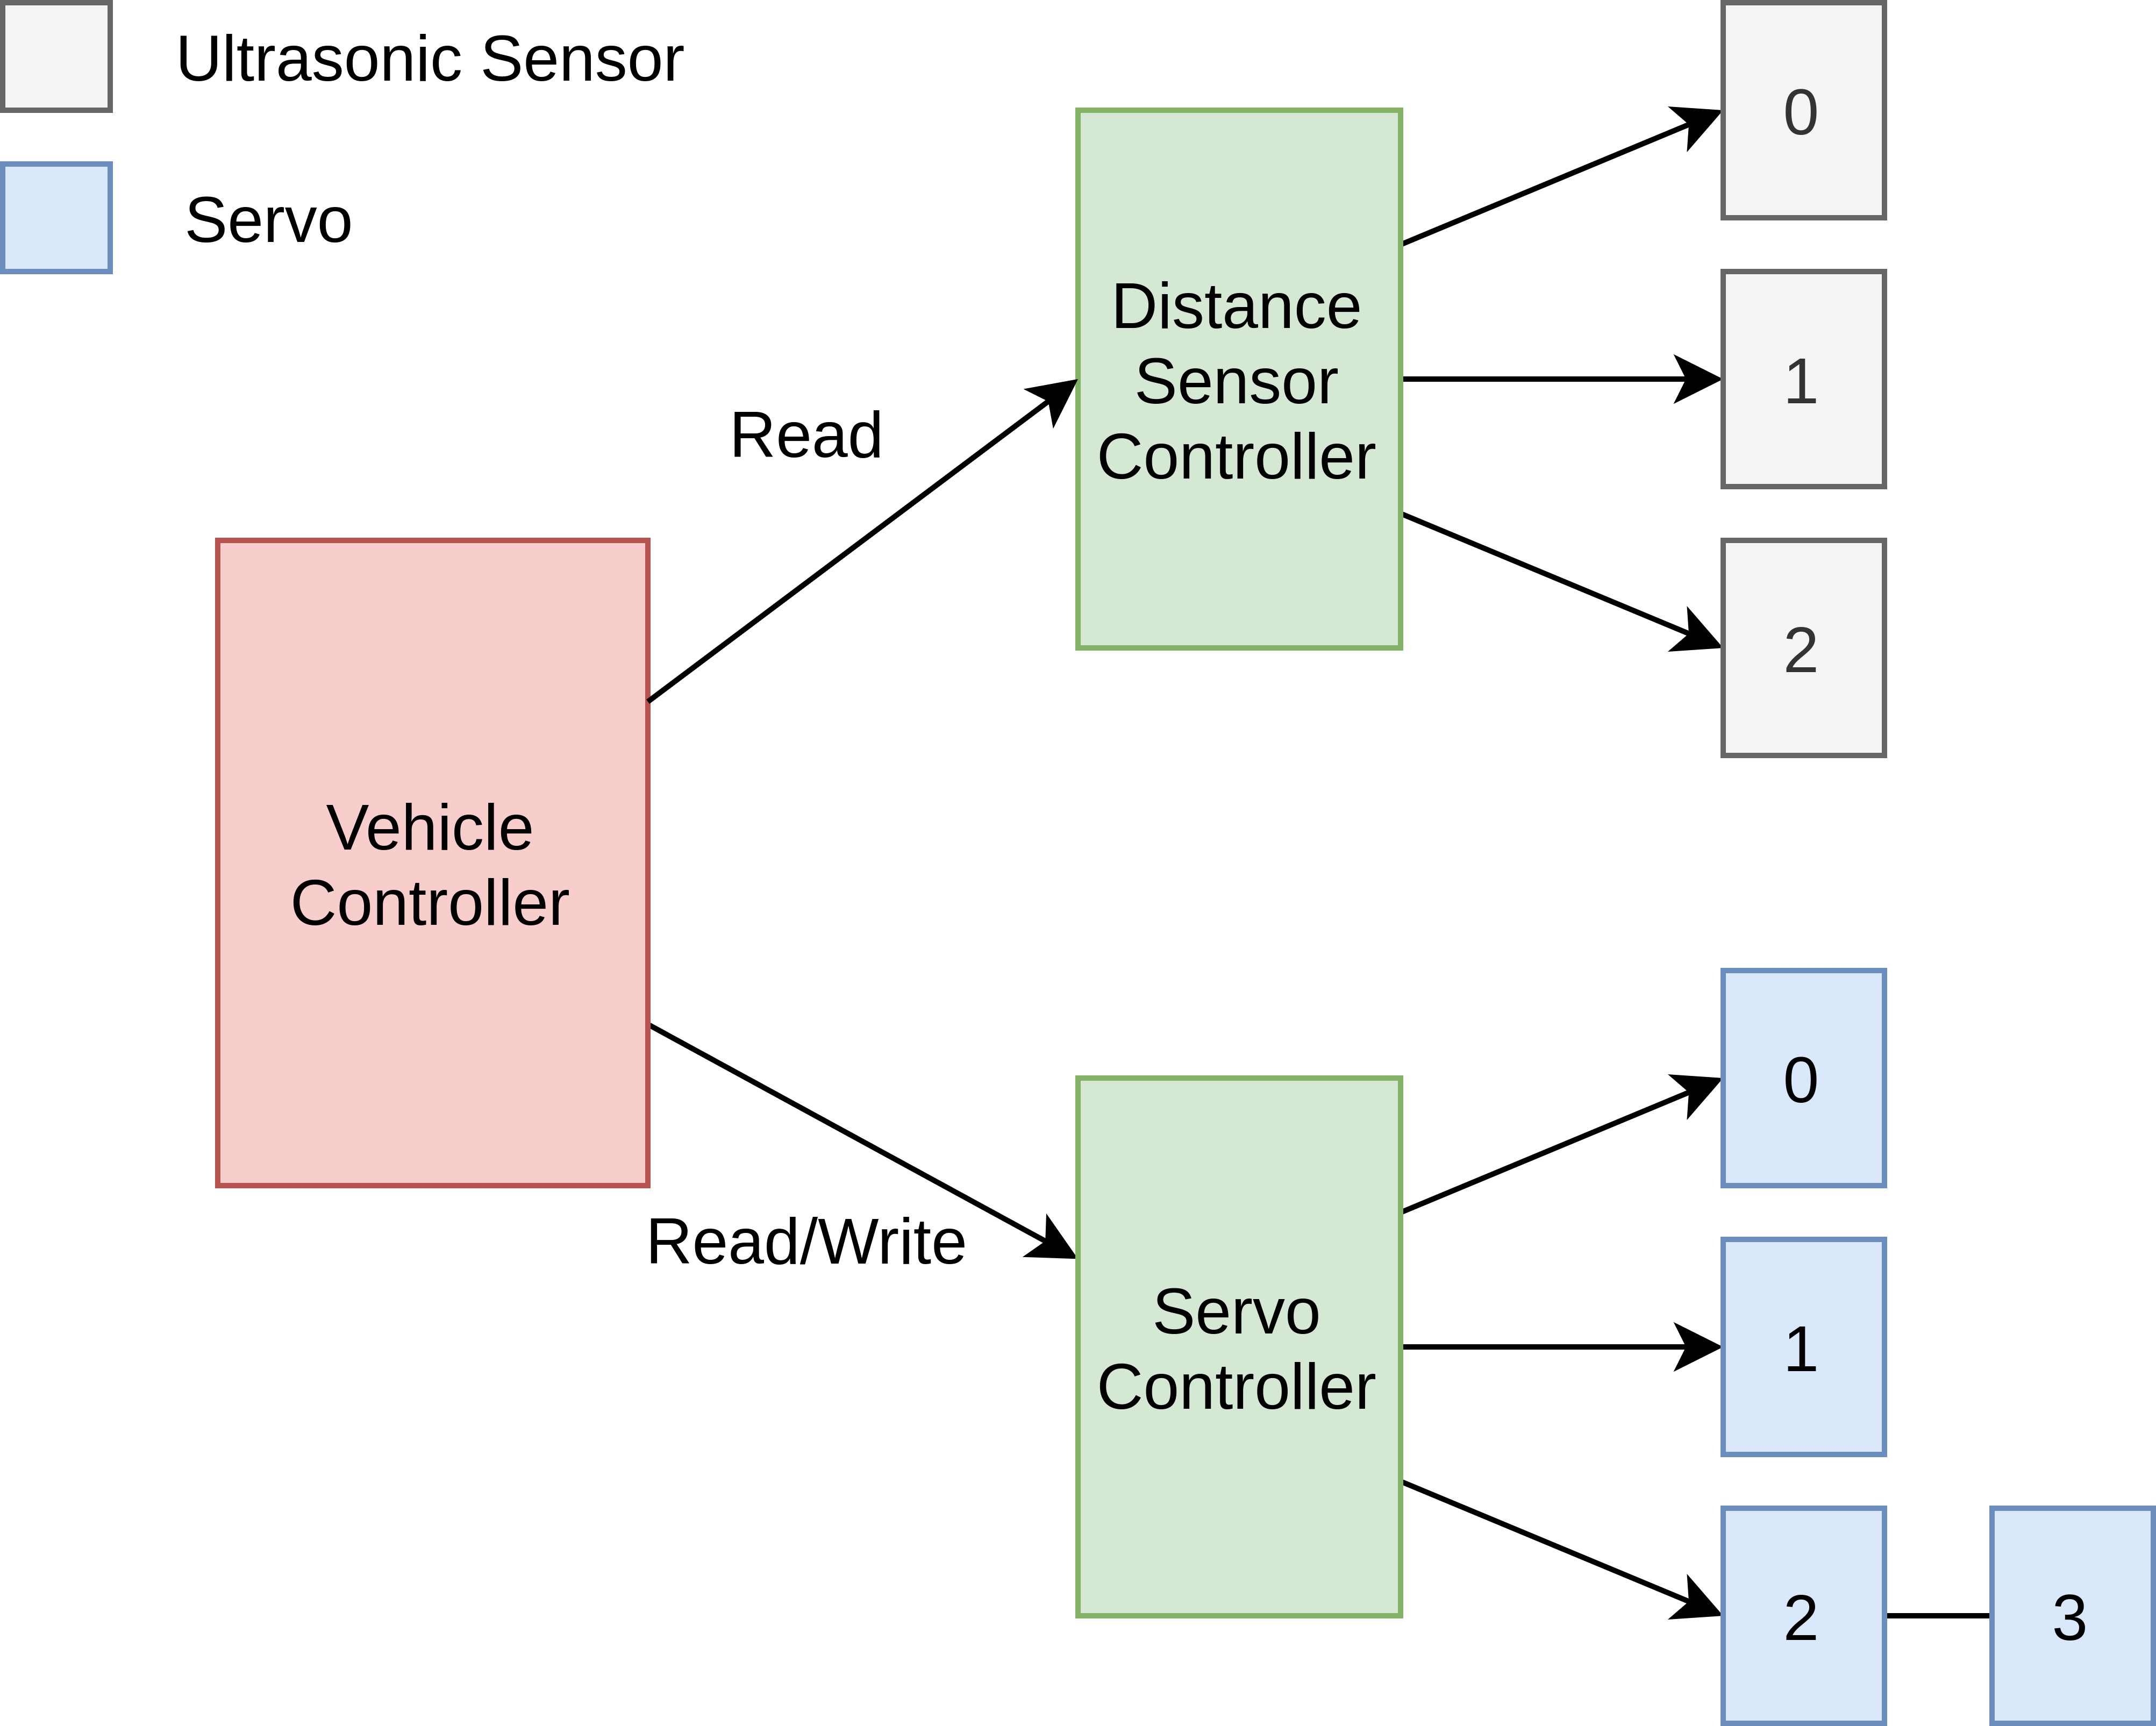
\includegraphics[width=\linewidth]{system-architecture.png}
	\caption{Block diagram of our system architecture}
	\label{SystemArchBlock}
\end{figure}


\begin{figure}[H]
	\centering
	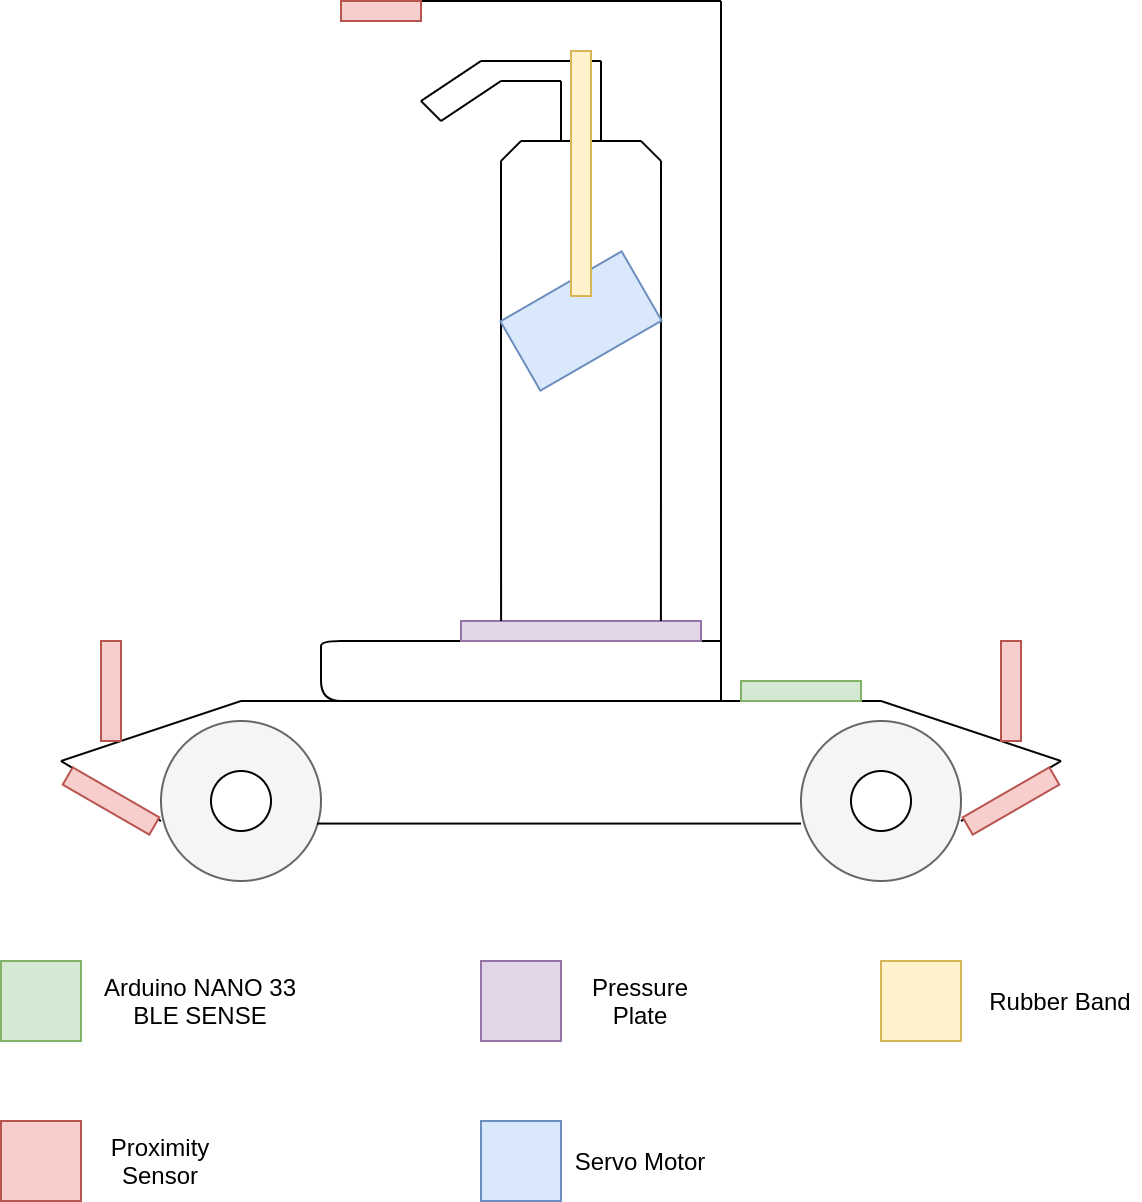
\includegraphics[width=\linewidth]{prototype-drawing.png}
	\caption{Prototype drawing of our vehicle}
	\label{ProtoDrawing}
\end{figure}

\newpage
%Referanse
\nocite{*}
\bibliographystyle{plain}
\bibliography{ref}
\addcontentsline{toc}{section}{References}

\newpage
\section{Maybe appendix}

\subsection{Stacktrace}
\lstset{frame=tb,
extendedchars = true,
texcl=true,
  language=Ada,
  aboveskip=3mm,
  belowskip=3mm,
  showstringspaces=false,
  columns=flexible,
  basicstyle={\small\ttfamily},
  numbers=none,
  numberstyle=\tiny\color{gray},
  keywordstyle=\color{black},
  commentstyle=\color{dkgreen},
  stringstyle=\color{mauve},
  breaklines=true,
  breakatwhitespace=true,
  tabsize=3
}
\begin{lstlisting}
# -*- asm -*- #############################
# Automatically generated by SVD2Ada
# For the nRF52840 reference description for radio MCU with ARM 32-bit Cortex-M4 Microcontroller  target
############################################

	.syntax unified
	.cpu cortex-m4
	.thumb

	.text
	.globl __vectors
	.p2align 8
__vectors:
	/* Cortex-M core interrupts */
	.word   0                    /* stack top address */
	.word   fault                /* 1 Reset.  */
	.word   fault                /* 2 NMI. */
	.word   fault                /* 3 Hard fault. */
	.word   fault                /* 4 Mem manage. */
	.word   fault                /* 5 Bus fault. */
	.word   fault                /* 6 Usage fault. */
	.word   fault                /* 7 reserved. */
	.word   fault                /* 8 reserved. */
	.word   fault                /* 9 reserved. */
	.word   fault                /* 10 reserved. */
	.word   __gnat_sv_call_trap  /* 11 SVCall. */
	.word   __gnat_bkpt_trap     /* 12 Breakpoint. */
	.word   fault                /* 13 reserved. */
	.word   __gnat_pend_sv_trap  /* 14 PendSV. */
	.word   __gnat_sys_tick_trap /* 15 Systick. */
	/* MCU interrupts */
	.word __gnat_irq_trap        /* 16 POWER_CLOCK */
	.word __gnat_irq_trap        /* 17 RADIO */
	.word __gnat_irq_trap        /* 18 UARTE0_UART0 */
	.word __gnat_irq_trap        /* 19 SPIM0_SPIS0_TWIM0_TWIS0_SPI0_TWI0 */
	.word __gnat_irq_trap        /* 20 SPIM1_SPIS1_TWIM1_TWIS1_SPI1_TWI1 */
	.word __gnat_irq_trap        /* 21 NFCT */
	.word __gnat_irq_trap        /* 22 GPIOTE */
	.word __gnat_irq_trap        /* 23 SAADC */
	.word __gnat_irq_trap        /* 24 TIMER0 */
	.word __gnat_irq_trap        /* 25 TIMER1 */
	.word __gnat_irq_trap        /* 26 TIMER2 */
	.word __gnat_irq_trap        /* 27 RTC0 */
	.word __gnat_irq_trap        /* 28 TEMP */
	.word __gnat_irq_trap        /* 29 RNG */
	.word __gnat_irq_trap        /* 30 ECB */
	.word __gnat_irq_trap        /* 31 CCM_AAR */
	.word __gnat_irq_trap        /* 32 WDT */
	.word __gnat_irq_trap        /* 33 RTC1 */
	.word __gnat_irq_trap        /* 34 QDEC */
	.word __gnat_irq_trap        /* 35 COMP_LPCOMP */
	.word __gnat_irq_trap        /* 36 SWI0_EGU0 */
	.word __gnat_irq_trap        /* 37 SWI1_EGU1 */
	.word __gnat_irq_trap        /* 38 SWI2_EGU2 */
	.word __gnat_irq_trap        /* 39 SWI3_EGU3 */
	.word __gnat_irq_trap        /* 40 SWI4_EGU4 */
	.word __gnat_irq_trap        /* 41 SWI5_EGU5 */
	.word __gnat_irq_trap        /* 42 TIMER3 */
	.word __gnat_irq_trap        /* 43 TIMER4 */
	.word __gnat_irq_trap        /* 44 PWM0 */
	.word __gnat_irq_trap        /* 45 PDM */
	.word __gnat_irq_trap        /* 46 IRQ 30. */
	.word __gnat_irq_trap        /* 47 IRQ 31. */
	.word __gnat_irq_trap        /* 48 MWU */
	.word __gnat_irq_trap        /* 49 PWM1 */
	.word __gnat_irq_trap        /* 50 PWM2 */
	.word __gnat_irq_trap        /* 51 SPIM2_SPIS2_SPI2 */
	.word __gnat_irq_trap        /* 52 RTC2 */
	.word __gnat_irq_trap        /* 53 I2S */
	.word __gnat_irq_trap        /* 54 FPU */
	.word __gnat_irq_trap        /* 55 USBD */
	.word __gnat_irq_trap        /* 56 UARTE1 */
	.word __gnat_irq_trap        /* 57 QSPI */
	.word __gnat_irq_trap        /* 58 CRYPTOCELL */
	.word __gnat_irq_trap        /* 59 IRQ 43. */
	.word __gnat_irq_trap        /* 60 IRQ 44. */
	.word __gnat_irq_trap        /* 61 PWM3 */
	.word __gnat_irq_trap        /* 62 IRQ 46. */
	.word __gnat_irq_trap        /* 63 SPIM3 */

	.text

	.thumb_func
.weak __gnat_irq_trap
.type __gnat_irq_trap, %function
__gnat_irq_trap:
0:	b 0b
	.size __gnat_irq_trap, . - __gnat_irq_trap

	.thumb_func
.weak __gnat_sv_call_trap
.type __gnat_sv_call_trap, %function
__gnat_sv_call_trap:
0:	b 0b
	.size __gnat_sv_call_trap, . - __gnat_sv_call_trap

	.thumb_func
.weak __gnat_pend_sv_trap
.type __gnat_pend_sv_trap, %function
__gnat_pend_sv_trap:
0:	b 0b
	.size __gnat_pend_sv_trap, . - __gnat_pend_sv_trap

	.thumb_func
.weak __gnat_sys_tick_trap
.type __gnat_sys_tick_trap, %function
__gnat_sys_tick_trap:
0:	b 0b
	.size __gnat_sys_tick_trap, . - __gnat_sys_tick_trap

	.thumb_func
fault:	b fault
\end{lstlisting}

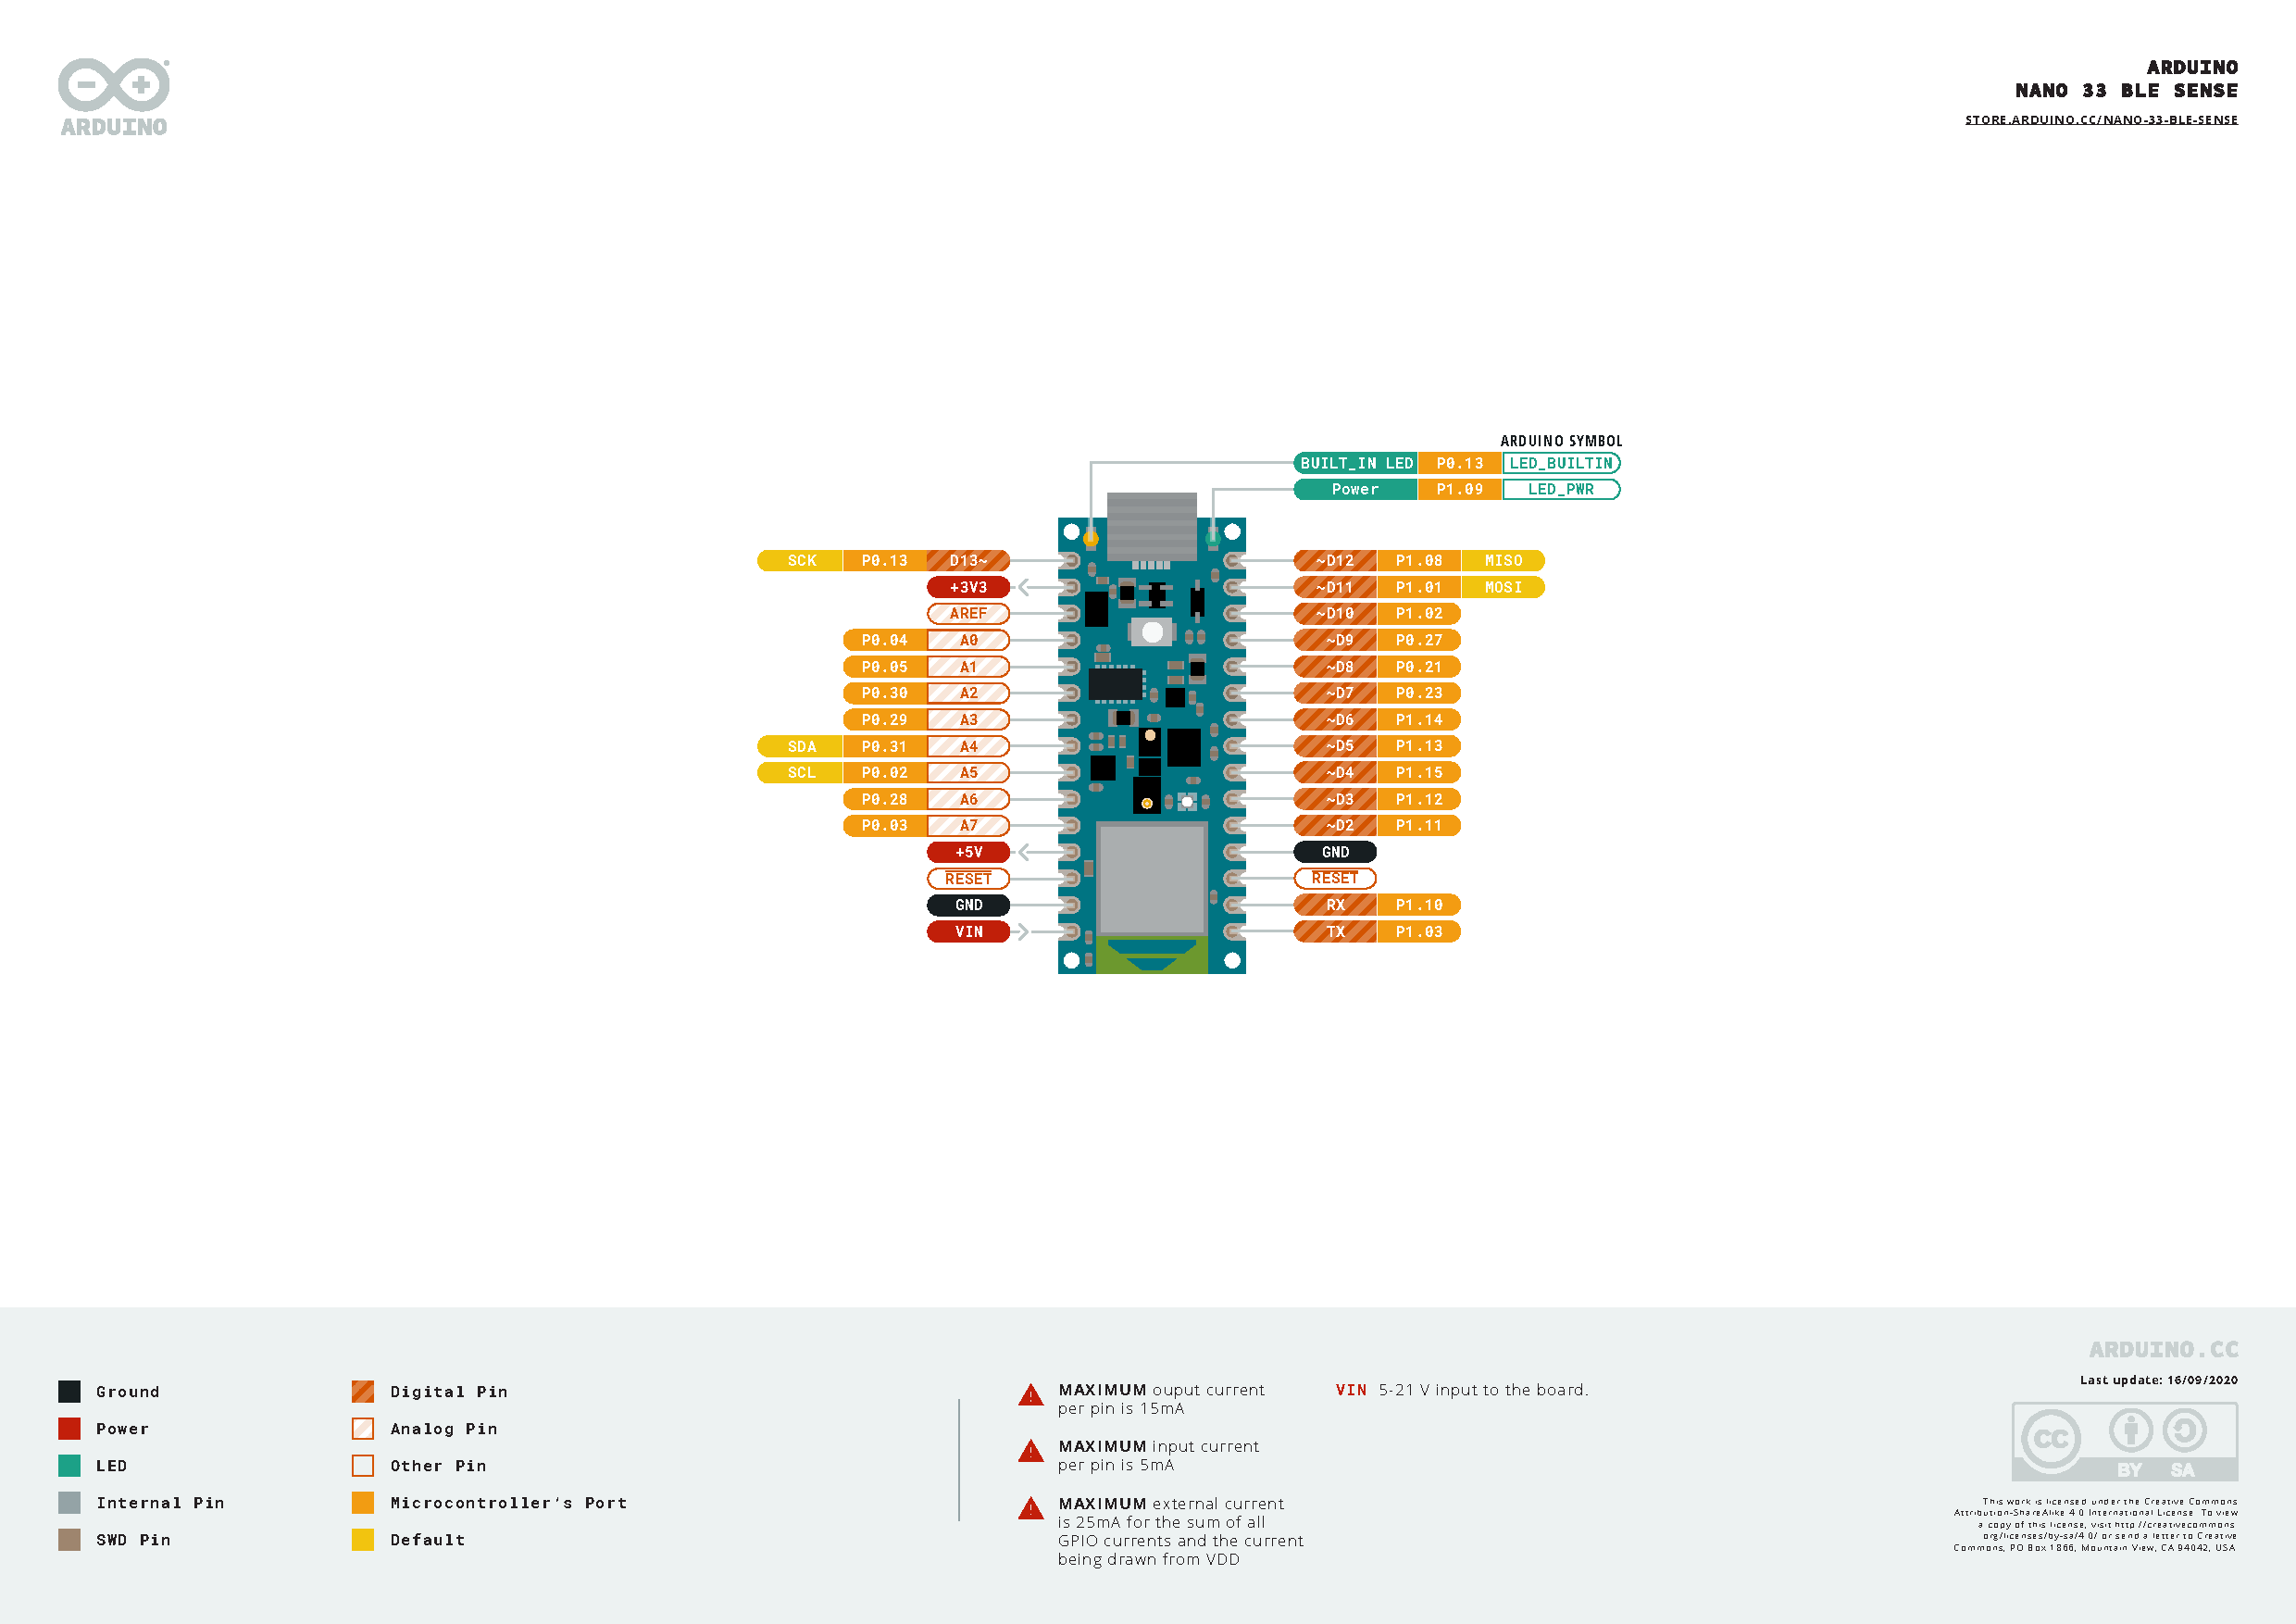
\includepdf[scale=1.0,pages=-,pagecommand=\subsection{Arduino Nano 33 BLE sense PIN layout\label{pinlayout}}]{pdf/Pinout-NANOsense_latest.pdf}

\end{document}

padding oracle attacks.
